%%This is a very basic article template.
%%There is just one section and two subsections.
\documentclass[11pt]{article}
\usepackage{times}
\usepackage{amsmath}
\usepackage{enumerate}

\usepackage{hyperref}
\usepackage[labelfont=bf]{subcaption}
\usepackage{graphicx,latexsym,float}
\usepackage{fancyhdr}
\usepackage{alltt}
\usepackage{listings}
\usepackage{epstopdf}
\usepackage{color}
\usepackage[labelfont=bf]{caption}
\usepackage{tabu}
\usepackage{xspace}
 
\usepackage{etoolbox}
%###
\makeatletter
\patchcmd{\@maketitle}{\begin{center}}{\begin{flushleft}}{}{}
\patchcmd{\@maketitle}{\end{center}}{\end{flushleft}}{}{}
\makeatother
%###
 
%set dimensions
\tabulinesep=1.2mm
\setlength{\textheight}{9.0in}
\setlength{\oddsidemargin}{0in}
\setlength{\evensidemargin}{0in}
\setlength{\topmargin}{-.50in}
\setlength{\textwidth}{6.5in}

\graphicspath{{./TechReportAndDocumentation_files/}}

\renewcommand{\lstlistingname}{Code Sample}

% For making java code look good
\definecolor{dkgreen}{rgb}{0,0.6,0}
\definecolor{gray}{rgb}{0.5,0.5,0.5}
\definecolor{mauve}{rgb}{0.58,0,0.82}

\lstset{frame=tb,
  language=Java,
  aboveskip=3mm,
  belowskip=3mm,
  showstringspaces=false,
  columns=flexible,
  basicstyle={\small\ttfamily},
  numbers=left,
  numberstyle=\tiny\color{gray},
  keywordstyle=\color{blue},
  commentstyle=\color{dkgreen},
  stringstyle=\color{mauve},
  breaklines=true,
  breakatwhitespace=true,
  tabsize=3
}

\begin{document}

\title{\vspace{-0.3in}{\bf \Huge RapidSmith 2 Introductory Exercises}}
\date{}
\maketitle
\vspace{-0.5in}

This document contains several introductory learning exercises to help new users
learn how to develop CAD tools in RapidSmith. Its goal is to help designers
become familiar with the following:

\begin{enumerate}
  \item How to use RapidSmith Device data structures (Tiles, Sites, BELs, etc.)
  \item How to use RapidSmith Design data structures (CellDesigns, Cells,
  CellNets, etc.)
  \item How to modify a RapidSmith netlist to add or remove logic
  \item How to Place and Route a logical netlist
  \item How to import Tincr Checkpoints into RapidSmith.
  \item How to export a RapidSmith netlist to a Tincr Checkpoint
\end{enumerate}

\noindent As you complete these exercises, read through the Tech Report
documentation and look through the example programs in
\textit{edu.byu.ece.rapidSmith.examples}.

\section{CLB Printer}
The purpose of this exercise is to gain a better understanding of the device
data structures in RapidSmith. Before starting, read the \textbf{Device} section
of the Tech Report in the RapidSmith repository. It gives a good overview of
Xilinx FPGA architecture and terminology, and introduces the RapidSmith data
structures that you will need for this task. As you work through this exercise,
it may be helpful to open the device browser in Vivado. Create a Java program
to do the following:

\begin{itemize}
  \item Load the Artix7 part ``xc7a100tcsg324-3'' into RapidSmith
  \item Find a tile of type ``CLBLL\_L'' in the device (this can be done by tile
  name, or getting all tiles in the device of type CLBLL\_L and choosing the
  first one).
  \begin{lstlisting}[numbers=none] 
  // Load the Artix7 device
  Device device = RSEnvironment.defaultEnv().getDevice("xc7a100tcsg324-3");

  // Get a handle to a Tile object
  Tile t = device.getTile("CLBLL_L_X2Y69");
  \end{lstlisting}
  \item Print the following information (in any format you want)
  \begin{itemize}
    \item The name of all Wires in the Tile
    \item The name and type of all Sites in the Tile
    \item For each Site, print the Site Pins, BELs, and Wires within the Site   
  \end{itemize}
  \item Create a function that takes as input a Wire object \textit{sourceWire}
  and an integer \textit{numHops}, and returns a list of Wires that are
  \textit{numHops} wires away from source wire. For example, if 1 is passed
  into the numHops parameter then all the wires directly connected to the
  source wire (through a PIP) should be returned. Only traversing a PIP wire
  connection counts as taking a hop.
  \begin{lstlisting}[numbers=none] 
  public Set<Wire> getWiresHops(Wire sourceWire, int numHops) {
	Set<Wire> sinkWires = new HashSet<Wire>();
	
	// Your code here
	
	return sinkWires;
  }
  \end{lstlisting}
\end{itemize}

\section{Design Printer}

The purpose of this exercise is to gain a better understanding of the design
data structures in RapidSmith. You will also learn how to load a Tincr
Checkpoint (which represents a Vivado design) into RapidSmith. Before starting,
read the \textbf{Designs} section of the Tech Report in the RapidSmith
repository. It gives a good overview of the netlist data structures and how to
use them. Create a Java program to do the following:

\begin{itemize}
  \item Load the \textit{cordic.tcp} Tincr checkpoint into RapidSmith (this
  design has been placed in Vivado, but not routed). This checkpoint is located
  in the \textit{exampleVivadoDesigns} directory of the repository.
  \item Print the following about the loaded design (in any format you want):
  \begin{itemize}
    \item The name of the design
    \item The number of cells and nets in the design
    \item For each cell, print its (1) name, (2) library cell type, (3) cell
    pins (with direction), (4) properties, and (5) BEL placement location (if
    any)
    \item For each net, print its (1) name, (2) net type, (3) source cell
    pin(s), and (4) all sink cell pins
  \end{itemize}
  \item Create a function to print a \texttt{CellNet}s INTERSITE route tree to
  the console in a meaningful way (it is a tree data structure so you will need
  to represent branching). Make sure to distinguish between PIP wire connections
  and non-PIP wire connections. Using your function, print the
  \texttt{RouteTree} for the net ``q\_OBUF[0]'' in the \textit{count16.tcp}
  design. Verify that it matches the route tree in \autoref{fig:routeTree}.
\end{itemize}

\begin{lstlisting}[numbers=none]
	// Load the count16.tcp checkpoint into RapidSmith
	String tcpPath = RSEnvironment.defaultEnv()
									.getEnvironmentPath()
									.resolve("exampleVivadoDesigns")
									.resolve("count16.tcp").toString();
	
	TincrCheckpoint tcp = VivadoInterface.loadTCP(tcpPath);
	CellDesign design = tcp.getDesign();
	CellNet net = design.getNet("q_OBUF[0]");
	
	// call your RouteTree function here
	printRouteTree(net);
	
	// optionally, you can print a graphical representation of the RouteTree for
	// comparison
	DotFilePrinter.getRouteTreeDotString(net); 
\end{lstlisting}

\begin{figure}[H]
\centering
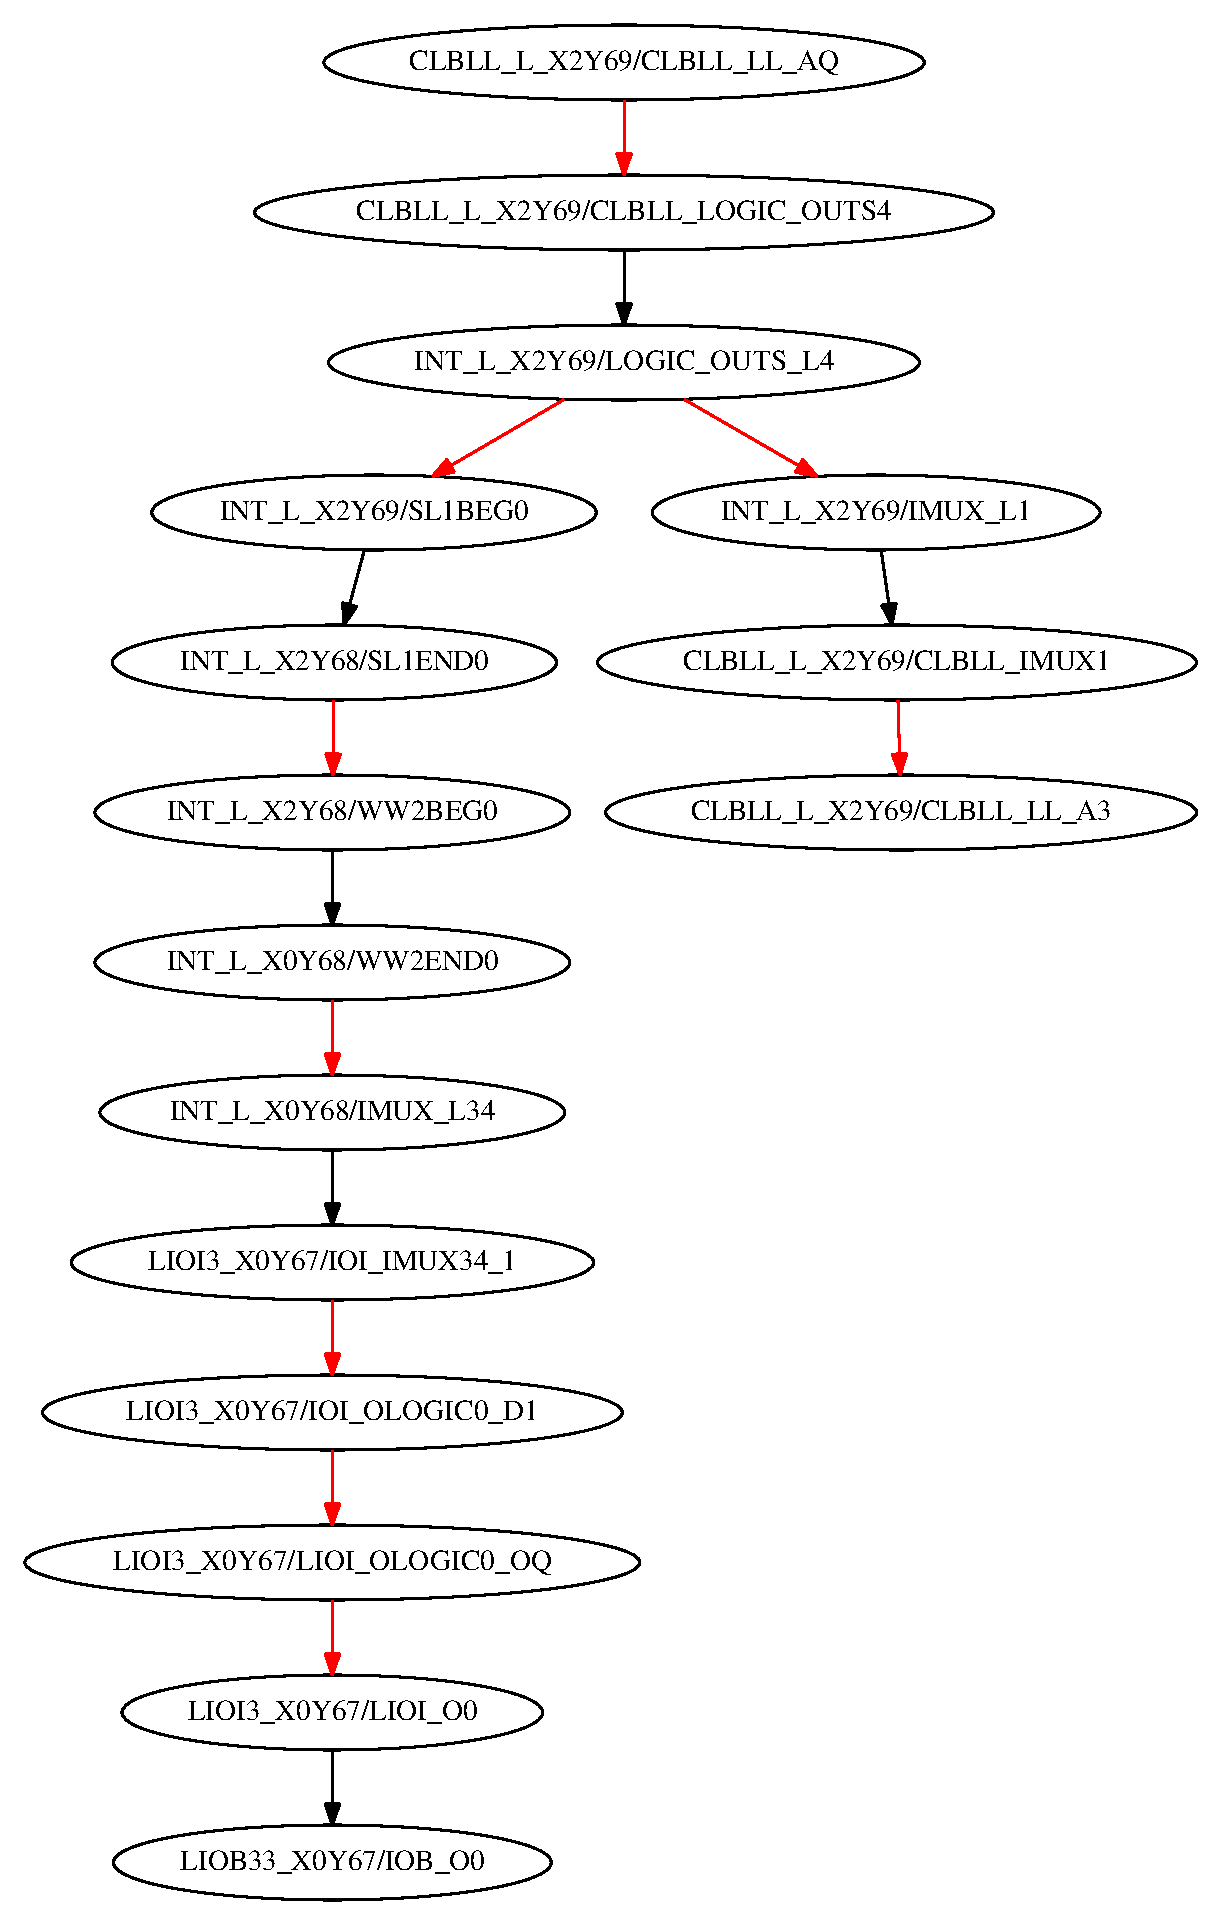
\includegraphics[width=0.6\columnwidth]{routeTreeTutorial.eps}
\caption{RouteTree visualization for the CellNet ``q\_OBUF[0]'' in the
\textit{count16.tcp} design. This can be used to verify that your RouteTree
printer function is working correctly.}
\label{fig:routeTree}
\end{figure}

\section{Full Adder} \label{sec:fullAdderNetlist}

The purpose of this exercise is to learn how to modify an existing netlist, or
create a new netlist from scratch. Using LUTs and FF cells (FDRE) in
RapidSmith, create a full adder circuit with registered outputs
(\autoref{fig:fullAdder}). Include a clock signal, but tie the reset signal on
the FF cells to ground. The Xilinx series7 CLB documentation
{\color{blue}{\url{https://www.xilinx.com/support/documentation/user_guides/ug474_7Series_CLB.pdf}}}
may be helpful to learn more about LUTs and FF BELs in Xilinx devices. Don�t
forget to create an input port cell (with an associated IBUF) for each of the
inputs, and an output port cell (with an associated OBUF) for each of the
outputs. To verify that the circuit is built correctly, create a dot file of
your netlist. 

\begin{lstlisting}[numbers=none]
// Use your function to create a full adder
CellDesign fullAdder = createFullAdder();

// Print a DOT file of your design
DotFilePrinter printer = new DotFilePrinter(fullAdder);
printer.printNetlistDotFile("fullAdder.dot");
\end{lstlisting}

\noindent To convert the generated DOT file into a viewable image, install
GraphViz {\color{blue}{\url{http://www.graphviz.org/}}} and run the following
command in a terminal:

\begin{verbatim}
dot -Tpng fullAdder.dot -o fullAdder.png
\end{verbatim}

\noindent Open the generated fullAdder.png image file, and visually verify that
you assembled the full adder correctly, and that the LUTs are correctly initialized.

\begin{figure}[H]
\centering
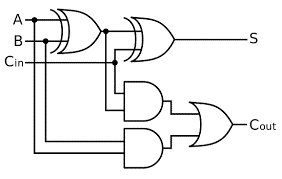
\includegraphics[width=0.6\columnwidth]{fullAdder.png}
\caption{Full Adder Schematic}
\label{fig:fullAdder}
\end{figure}

\section{Placing the Full Adder}
Using the full adder circuit you created in \autoref{sec:fullAdderNetlist},
place the design onto a Artix7 \textit{xc7a100tcsg324} Xilinx part. This can be
done in three different ways:

\begin{enumerate}
  \item Manually place all cells
  \item Randomly place all cells
  \item Implement a placement algorithm.
\end{enumerate}

\noindent It is suggested that new users start with method 1, and move onto
method 2 and 3 as they get more experience with RapidSmith. \textbf{NOTE:}
placing cells onto BELs is actually a packing problem. Placement is usually done
at Site boundaries.

\section{Automated Router}
Design a simple algorithm to automatically route the INTERSITE portion of a
CellNet using RouteTrees. Initially, your algorithm should only route
\textbf{one sink pin} of the net. Once this works, modify your algorithm to
route all sinks of a net. To test your algorithm, load the \textit{cordic.tcp}
checkpoint into RapidSmith, route the net named
``u2/gen\_pipe[8].Pipe/Zo\_reg\_n\_0\_[9]'', and generate a TCL command that
can highlight the used wires in Vivado (shown below).

\begin{lstlisting}[numbers=none]
// Load the count16.tcp checkpoint into RapidSmith
String tcpPath = RSEnvironment.defaultEnv()
								.getEnvironmentPath()
								.resolve("exampleVivadoDesigns")
								.resolve("cordic.tcp").toString();

TincrCheckpoint tcp = VivadoInterface.loadTCP(tcpPath);
CellDesign design = tcp.getDesign();
CellNet net = design.getNet("u2/gen_pipe[8].Pipe/Zo_reg_n_0_[9]");

// Call your router
RouteTree route = routeNet(net);

// Print a TCL command to the console for testing
System.out.println(RapidSmithDebug.createHighlightWiresTclCommand(route));
\end{lstlisting}

\noindent Load the equivalent DCP file into Vivado
(\textit{exampleVivadoDesigns/cordic.dcp}), and copy the Tcl command generated
above into the Tcl console. This will highlight all of the wires that your
router used when completing the route. Visually verify that your route starts at
the correct source site pin, and ends at the correct sink site pins.
  
\end{document}
